%-------------------------------------------------------------------------------
\chapter{Implementation of a Walking Module for Nao}
\label{ch.naomodule}
%-------------------------------------------------------------------------------
During the work on the thesis two solvers for \ac{MPCWMG}, a simple footstep pattern
generator, an inverse kinematics library, and a walking module for Nao robots were 
developed\footnote{All sources are publicly available at \url{https://github.com/asherikov/}.}. 
Instructions on compilation and installation are distributed with the sources.

The architecture of the walking module is schematically depicted in \cref{fig.arch}.

\begin{figure}[ht]
    \centerline{%
    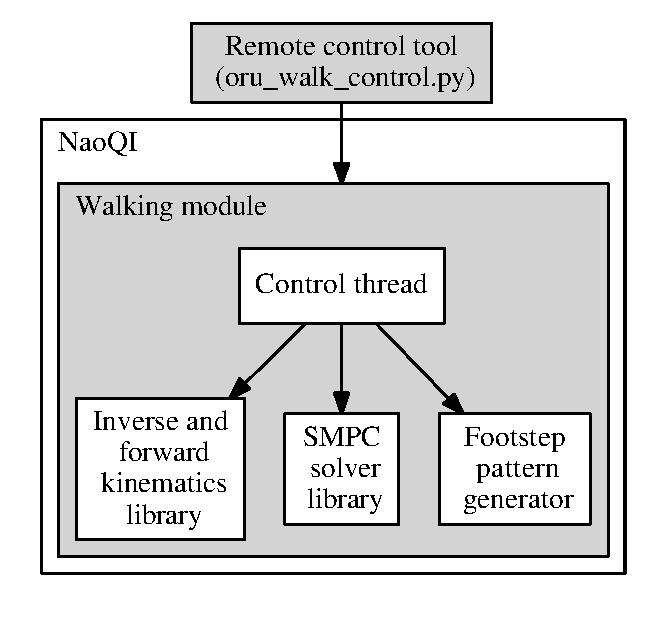
\includegraphics[scale=0.6]{Figures/nao_mod_arch.eps}}
    \caption{Architecture of the walking module}
    \label{fig.arch}
\end{figure}

The walking module runs within the \verb|NaoQI| framework on a Nao robot. Commands 
are sent to the module using a simple command line control tool from a personal 
computer.

When walk is started the module reads parameters from a configuration file and
spawns a control thread, which is periodically activated in order to determine
the joint commands. The necessary joint angles are determined based on the 
desired position of the \ac{CoM} and poses of the feet provided by \ac{MPCWMG}
solvers and footstep pattern generator, respectively. The functions of each submodule
are described in more detail in this chapter.

Note that some implementations \cite{NaoWalk} assume that the \ac{CoM} is fixed to 
the torso, hence the trajectory of the \ac{CoM} is tracked by some point on the
torso. We do not make such assumption and control the real \ac{CoM}.



%%%%%%%%%%%%%%%%%%%%%%%%%%%%%%%%%%%%%%%%%%%%%%%%%%%%%%%%%%%%%%%%%%%%%%%%%%%%%%%%%%
%%%%%%%%%%%%%%%%%%%%%%%%%%%%%%%%%%%%%%%%%%%%%%%%%%%%%%%%%%%%%%%%%%%%%%%%%%%%%%%%%%
%%%%%%%%%%%%%%%%%%%%%%%%%%%%%%%%%%%%%%%%%%%%%%%%%%%%%%%%%%%%%%%%%%%%%%%%%%%%%%%%%%
\section{Sparse MPC Solver}
The purpose of the \ac{MPCWMG} is to generate a trajectory for the \ac{CoM}. To be
precise, a trajectory for the \ac{ZMP} is generated first, then the \ac{CoM}
positions are computed from it. The trajectories are shown in \cref{fig.footsteps}.
In order to generate trajectories the reference \ac{ZMP} points must be given,
in \ac{SS} they are placed in the middle of the constraining rectangle, in a \ac{DS} 
the reference \ac{ZMP} point of the closest \ac{SS} is used.

\begin{figure}[ht]
    \centerline{%
    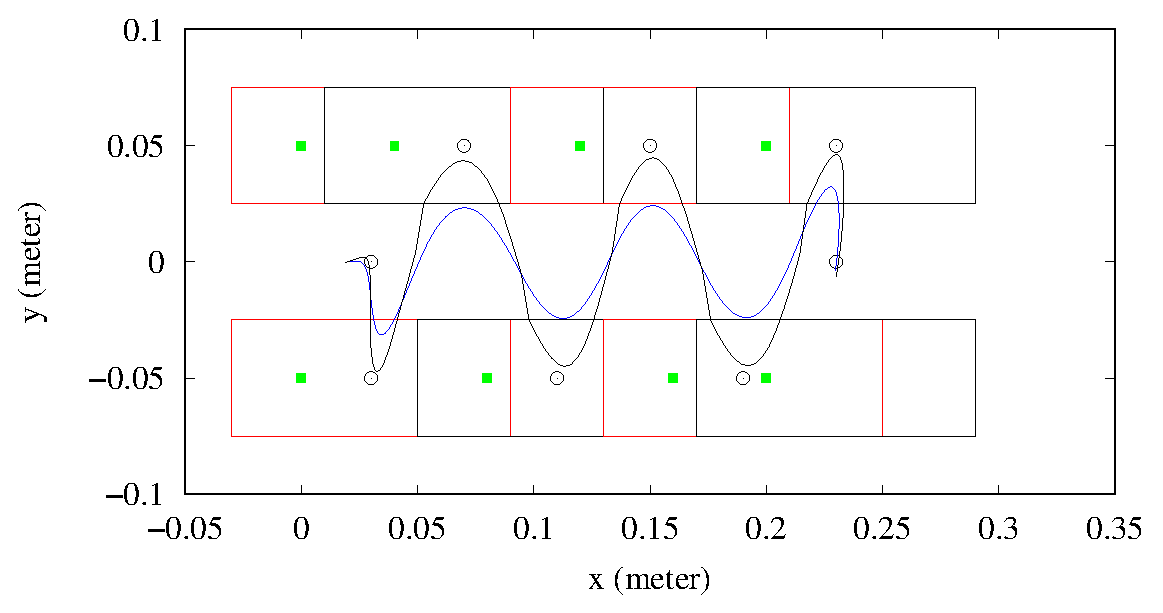
\includegraphics[scale=0.5]{Figures/sim_nodist_as.eps}}
    \caption[Footsteps and trajectories of {\bf CoM} and {\bf ZMP}]{Red and black rectangles
    represent \ac{SS}, \ac{DS} are omitted. Blue and black curves show trajectories 
    of \ac{CoM} and \ac{ZMP}, respectively. Black circles stand for reference 
    \ac{ZMP} positions. Green boxes are the footstep reference points. The data was obtained
    during simulation.}
    \label{fig.footsteps}
\end{figure}

Both active set (\cref{sec.as}) and logarithmic barrier (\cref{sec.ip}) 
methods were developed for solving the \ac{QP}. One of them can be 
selected by appropriately setting options in the configuration file. In particular,
these options can be used to control the mechanisms that limit the execution
time of the solver. The execution time of active set method can be controlled 
by imposing a limit on the number of activated constraints and disabling the 
deactivation of constraints. The number of iterations of the logarithmic barrier
method can be also explicitly limited.


%%%%%%%%%%%%%%%%%%%%%%%%%%%%%%%%%%%%%%%%%%%%%%%%%%%%%%%%%%%%%%%%%%%%%%%%%%%%%%%%%%
%%%%%%%%%%%%%%%%%%%%%%%%%%%%%%%%%%%%%%%%%%%%%%%%%%%%%%%%%%%%%%%%%%%%%%%%%%%%%%%%%%
%%%%%%%%%%%%%%%%%%%%%%%%%%%%%%%%%%%%%%%%%%%%%%%%%%%%%%%%%%%%%%%%%%%%%%%%%%%%%%%%%%
\section{Footstep Pattern Generator}
The functionality of the footstep pattern generator is two-fold. It provides
functions to predefine footsteps and generate swing foot trajectories during 
walk.

The positions and orientations of the footsteps must be defined before walk is
started, an example of footstep sequence is depicted in \cref{fig.footsteps}. 
% Automatic footstep generation was left out of the scope of this thesis. TODO

\begin{figure}[ht]
    \centerline{%
    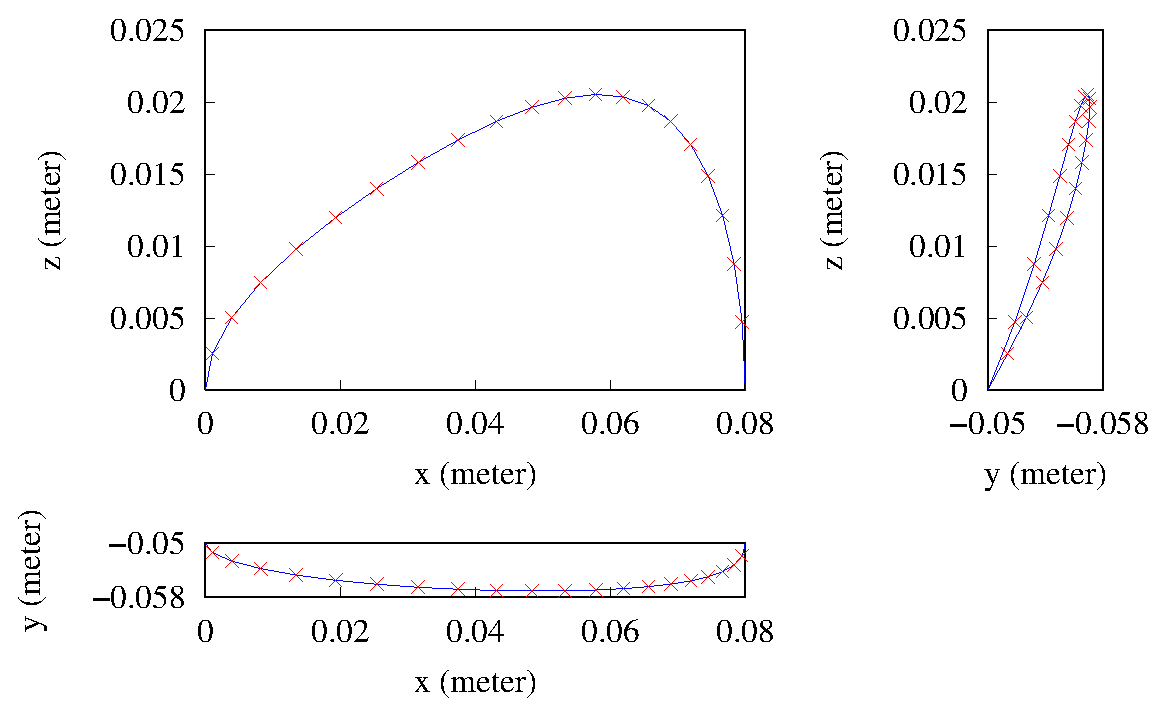
\includegraphics[scale=0.5]{Figures/foottraj.eps}}
    \caption[Swing foot trajectory]{Right swing foot trajectory in three
    projections. Red crosses show points that correspond to sampling intervals
    of $20$ milliseconds. The data was obtained during simulation.}
    \label{fig.foottraj}
\end{figure}

The foot trajectories are generated using Bezier curves. Parameters for the curves
were found experimentally. The three projections of a right foot trajectory produced
during straight walk are shown in \cref{fig.foottraj}, the trajectory of the left 
foot is symmetric.



%%%%%%%%%%%%%%%%%%%%%%%%%%%%%%%%%%%%%%%%%%%%%%%%%%%%%%%%%%%%%%%%%%%%%%%%%%%%%%%%%%
%%%%%%%%%%%%%%%%%%%%%%%%%%%%%%%%%%%%%%%%%%%%%%%%%%%%%%%%%%%%%%%%%%%%%%%%%%%%%%%%%%
%%%%%%%%%%%%%%%%%%%%%%%%%%%%%%%%%%%%%%%%%%%%%%%%%%%%%%%%%%%%%%%%%%%%%%%%%%%%%%%%%%
\section{Inverse and Forward Kinematics Library}\label{sec.ik}
Inverse and forward kinematics library provide functions that solve \ac{FK} and \ac{IK}.
In the sources it is also referred to as \ac{IGM}, where the word ``geometrical'' is used 
instead of ``kinematics'' to emphasize, that the library works with positions of actuators 
and not with their motions.


%%%%%%%%%%%%%%%%%%%%%%%%%%%%%%%%%%%%%%%%%%%%%%%%%%%%%%%%%%%%%%%%%%%%%%%%%%%%%%%%%%
\subsection{Algorithms}\label{sec.ik_alg}
From a mechanical point of view a humanoid robot is a chain of $n+1$ rigid bodies
({\bf links}) connected by $n$ {\bf joints}. One of the extremities of this chain 
is often referred to as the base and some of the others as end-effectors. Motions 
of a robot are compositions of elementary motions of links with respect to each 
other. Motion can be represented in two spaces: {\bf joint space} and {\bf operational 
space}, in the former one the coordinates are $n$ joint angles, in the latter -- 
positions and orientations of end-effectors with respect to the base. Joint and 
operational spaces are related by \ac{FK} and \ac{IK}.

Let $\mbm{q} \in \RR^n$ be the joint space coordinates, and $\mbm{r} \in \RR^m$ be 
the operational space coordinates.

The purpose of the \ac{FK} is determination of position and orientation 
of a frame attached to an end-effector given the reference frame attached to the base
of the chain and a set of joint angles. It is performed by solving
$$
\mbm{r} = f_r(\mbm{q}).
$$

The \ac{IK} problem is opposite to the \ac{FK} problem. \ac{IK} finds the set of joint 
angles that realizes the desired pose of an end-effector using inverse function of $f_r$
$$
\mbm{q}=f_r^{-1}(\mbm{r}).
$$

There are two approaches to solve the \ac{IK} problem: analytical (closed-form) and 
numerical. The \ac{IK} is a typical nonlinear problem and it is not always possible to 
find a closed-form solution. In such cases numerical methods can be used instead.
A numerical solution of \ac{IK} can be found in a several ways using different iterative
schemes. The implementation of \ac{IK} for Nao used in our work is similar to the method 
described in \cite{ZhangIKRep}.

The Taylor approximation of the \ac{FK} function can be expressed as
\begin{equation}\label{eq.ik_taylor}
\mbm{r} = f_r(\mbm{q}) \approx f_r(\mbm{q}_k) + \mbm{J}_r(\mbm{q}_k)(\mbm{q}-\mbm{q}_k),
\end{equation}
%
where $\mbm{q}_k$ is the initial approximation of the solution, and $\mbm{J}_r$ is the
$m \times n$ Jacobian matrix, whose computation is described in detail in 
\cite{AntonioThesis}. Let $\mbm{e}_r = \mbm{r} - f_r(\mbm{q}) = f_r(\mbm{q}_k)$ 
and $\Delta\mbm{q} = \mbm{q}-\mbm{q}_k$, then from \cref{eq.ik_taylor} we obtain
%
\begin{equation}\label{eq.ik_eqc}
\mbm{e}_r = \mbm{J}_r(\mbm{q}_k)\Delta\mbm{q},
\end{equation}

Consider the optimization problem
\begin{equation}\label{eq.ik_opt}
\begin{split}
\minimize{\Delta\mbm{q} \in \mathbb{R}^n} 
            & \frac{1}{2} \norm{ \Delta\mbm{q} + \mbm{e}_q}^2_{\mbm{H}} \\
\subjectto  & \mbm{e}_r = \mbm{J}_r(\mbm{q}_k)\Delta\mbm{q},
\end{split}
\end{equation}
where $\mbm{e}_q = \mu_{ik} (\mbm{q}_k - \mbm{q}_0)$ is the weighted difference between the 
initial guess and the reference joint angles $\mbm{q}_0$. $\mbm{e}_q$ is added to the 
objective function in order to obtain repetitive solutions.

The optimization problem~\eqref{eq.ik_opt} is equivalent to
\begin{equation}\label{eq.ik_opt_final}
\begin{split}
\minimize{\Delta\mbm{q} \in \mathbb{R}^n} 
            & \frac{1}{2} \norm{ \Delta\mbm{q} }^2_{\mbm{H}} + \mbm{e}_q^T \mbm{H} \Delta\mbm{q} \\
\subjectto  & \mbm{e}_r = \mbm{J}_r(\mbm{q}_k)\Delta\mbm{q}.
\end{split}
\end{equation}



%%%%%%%%%%%%%%%%%%%%%%%%%%%%%%%%%%%%%%%%%%%%%%%%%%%%%%%%%%%%%%%%%%%%%%%%%%%%%%%%%%
\subsection{Implementation}
The support foot is selected as the fixed base of the kinematic tree. Consequently,
the base must be periodically changed. This change is performed in the end of \ac{DS}
and is a source of error, that must be accounted for (see Section 
\cref{sec.err_feedback}). In theory, it is possible to always use the same foot as 
the base assuming that the position tracking for this foot is perfect, but this 
assumption is admissible only in simulation. 

Alternatively, the torso can be selected as the base \cite{NaoWalk}. Due to implicit
error feedback it might a better choice when a robot is subject to disturbances.
%For example, consider a situation when a robot is held back by a wall. If 
%one foot is chosen as the base, the robot tries to bring the \ac{CoM} through the 
%wall and fails. On the other hand, if the torso is the base, then 

The functions that solve \ac{FK}, compute the Jacobian $\mbm{J}_r$ and $\mbm{e}_r$
were generated using \verb|Maple|\footnote{The code is available as well 
at \url{https://github.com/asherikov/}.}. 

Two \ac{FK} functions are used. The first one determines pose of a swing foot, when 
change of the base is performed. The second computes the \ac{CoM} position for error 
feedback.
%, it requires knowledge of the poses and \ac{CoM}s of all links is necessary.

The \ac{QP}~\eqref{eq.ik_opt_final} is solved using block elimination with $\mbm{H} = 
\mbm{I}$, and $\mu_{ik}$ was determined experimentally. The problem is resolved until 
the change in joint angles becomes smaller than the minimal angle detected by the 
joint position sensors. Also, a limit on the number of iterations is imposed to 
detect cases, when there is no solution.

\begin{figure}[ht]
    \centerline{%
    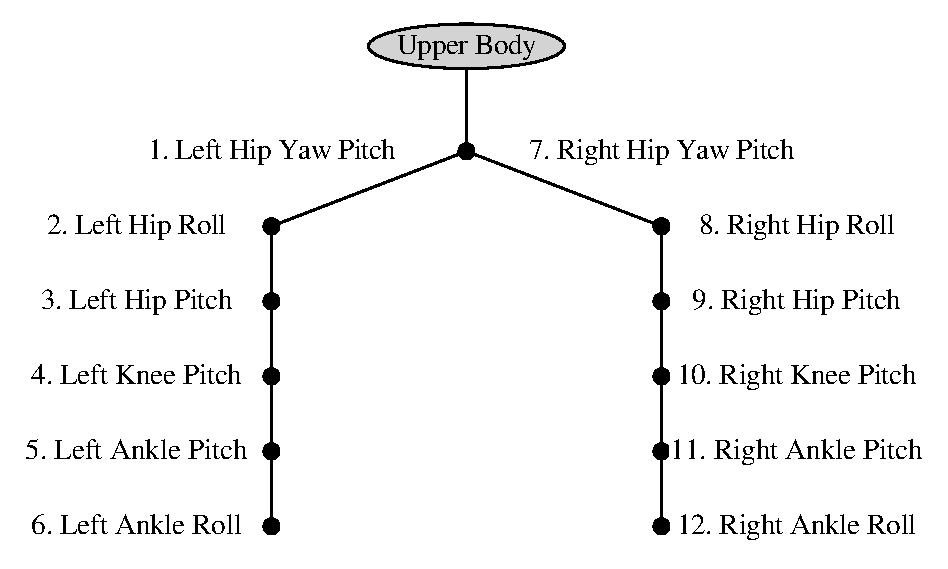
\includegraphics[scale=0.6]{Figures/nao_joints.eps}}
    \caption{Lower body joints of Nao}
    \label{fig.joints}
\end{figure}

The joint angles of the upper body are fixed, hence only $12$ lower body joints depicted 
in \cref{fig.joints} are controlled. Note that joints $1$ and $7$ are coupled
\footnote{Refer to \url{http://www.aldebaran-robotics.com/documentation/index.html} for
more information.}, that is, they share the same motor and move simultaneously and 
symmetrically. In the case of conflicting orders \verb|LHipYawPitch| always takes priority. 
The coupling between these joints is handled by imposing an equality constraint 
$\Delta\mbm{q}_1 = \Delta\mbm{q}_7$. It is also possible to reduce the number of controlled 
joints to account for this. 

The total number of imposed constraints is $10$:
\begin{itemize}
    \item $3$ on the position of the swing foot;
    \item $3$ on the orientation of the swing foot;
    \item $3$ on the position of the \ac{CoM};
    \item $1$ to take into account the coupled joint.
\end{itemize}

Several alternative versions of \ac{IK} implementation were also tested. In the early 
variants of the \ac{IK} module the difference between the joint angles and the reference 
angles is not penalized, but the constraints on the orientation of the frame fixed to 
the \ac{CoM} are used instead. These constraints are imposed in such a way, that the 
rotation about $x$ and $y$ axes is not allowed. The constraint on rotation about $x$ 
axis was removed in order to reduce the load on the \verb|HipRoll| joints, which tend 
to violate their limits for some \ac{CoM} trajectories otherwise. Further experiments 
demonstrated, that the gait is better, when there are no constraints on the orientation 
of the \ac{CoM}. Also, it is unclear how to define the desired orientation of the \ac{CoM} 
in a general case, for example, during a circular walk. The penalization of the 
difference with the reference joint angles was introduced to maintain upright posture
and avoid failures due to bad configurations of the lower body joints.

Another version of \ac{IK} is similar to the current one, but it controls all joints of 
the robot instead of only the lower body joints. However, the ability to cope with external 
disturbances is roughly the same. Furthermore, this approach requires more time for 
computations.

%It is assumed that the leading matrix of the constraints is nonsingular.



%%%%%%%%%%%%%%%%%%%%%%%%%%%%%%%%%%%%%%%%%%%%%%%%%%%%%%%%%%%%%%%%%%%%%%%%%%%%%%%%%%
%%%%%%%%%%%%%%%%%%%%%%%%%%%%%%%%%%%%%%%%%%%%%%%%%%%%%%%%%%%%%%%%%%%%%%%%%%%%%%%%%%
%%%%%%%%%%%%%%%%%%%%%%%%%%%%%%%%%%%%%%%%%%%%%%%%%%%%%%%%%%%%%%%%%%%%%%%%%%%%%%%%%%
\section{Control Thread}
The logic of one control loop of the control thread is shown in \cref{fig.seq}. 

\begin{figure}[ht]
    \centerline{%
    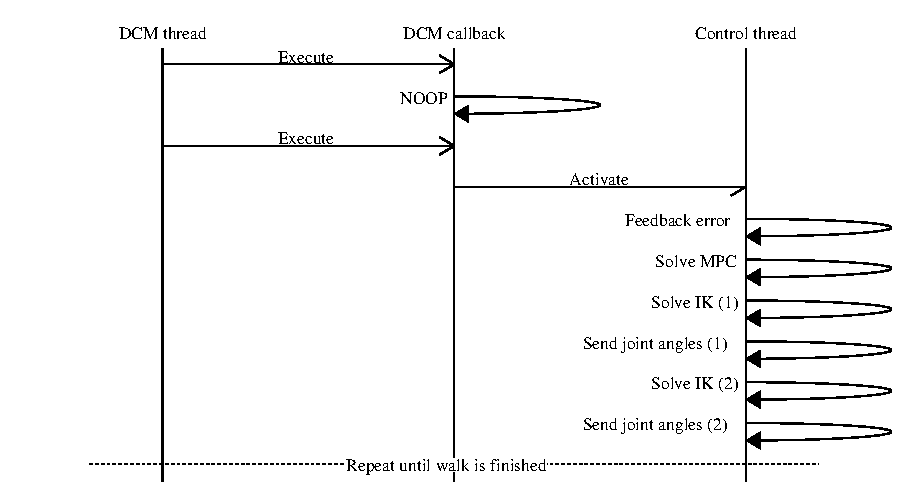
\includegraphics[scale=0.8]{Figures/nao_mod_seq.eps}}
    \caption{Control loop of the walking module}
    \label{fig.seq}
\end{figure}


%%%%%%%%%%%%%%%%%%%%%%%%%%%%%%%%%%%%%%%%%%%%%%%%%%%%%%%%%%%%%%%%%%%%%%%%%%%%%%%%%%
\subsection{Real-time Control Features of the Nao API}
The control of a walking robot must be performed in real-time. \ac{API} of a Nao
robots provides two possible ways to implement this. The first one is to register 
callback function from \ac{DCM}, which is activated each $10$ milliseconds. The main
purpose of the \ac{DCM} is to update sensor readings in the memory, since there is
no direct access to the sensors. The second way is to register callback function 
from the built-in \verb|Motion| module, which is activated each $20$ milliseconds. 
The \verb|Motion| module can perform walk and other operations, but it is activated
even if no commands were sent. 

We have tried to use both methods for real-time control. Experiments have 
demonstrated, that period of $10$ milliseconds is too short to perform all necessary 
operations. On the other hand, when the callback from \verb|Motion| module was
used, it was observed, that the sensor readings are not necessary updated twice
during the $20$ milliseconds between activations of the module (at least in the
simulation on a personal computer). Hence, a control thread was introduced, which 
is activated by a callback function that is called when \ac{DCM} finishes its work. 
Thus the callback function is executed each $10$ milliseconds. It has a counter of 
executions, and on each even execution (that is, each $20$ milliseconds) it wakes up 
the control thread using a synchronization tool provided by the \verb|Boost| library. 

The priority of the control thread plays a critical role, since sometimes it is not 
possible to complete all necessary computations in available time using the default 
priority. We use \verb|SCHED_FIFO| scheduling policy, the same as \ac{DCM} thread 
uses. The priority is set to $65$. Note that \verb|NaoQi| does not run with root 
privileges and priority cannot be set arbitrarily. 


%%%%%%%%%%%%%%%%%%%%%%%%%%%%%%%%%%%%%%%%%%%%%%%%%%%%%%%%%%%%%%%%%%%%%%%%%%%%%%%%%%
\subsection{Error Feedback}\label{sec.err_feedback}
On the feedback step the position of the \ac{CoM} is computed based on the current
joint angles. Then the error between the computed and the expected positions of
the \ac{CoM} is computed. The expected position is taken from the previous solution
of \ac{MPCWMG}. If the error is below a given threshold, it is silently discarded,
otherwise it is scaled by a gain and added to the expected position of the \ac{CoM}. 
Error feedback for the velocity and acceleration of the \ac{CoM} is not performed. 
The state obtained after error feedback is used as initial state of the \ac{MPCWMG}.

There is also a second type of error feedback, which is performed when the reference
foot is changed. Note that when the new reference foot touches the ground its position
is not exactly the same as the target one. Therefore, if the reference frame is
moved to this foot, an error in position of \ac{CoM} appears. To avoid this effect the
footstep pattern generator is informed about the error in foot position before the
reference foot is changed. It is also necessary to synchronize joint angles in the 
model of the robot, which is used in inverse kinematics library, with the joint angles 
obtained from sensors.


%%%%%%%%%%%%%%%%%%%%%%%%%%%%%%%%%%%%%%%%%%%%%%%%%%%%%%%%%%%%%%%%%%%%%%%%%%%%%%%%%%
\subsection{Accounting for the Computational Delay}\label{sec.mpc_delay}
Quadratic programming is a time demanding task, and it takes a considerable part of 
one control sampling period. It is impossible to obtain smooth joint motions without 
accounting for the computational delay. The model of the system can be modified for 
this purpose as described in Section $2.5$ of \cite{MacMPC}. However, for the sake 
of simplicity the system was not modified, and a heuristic described in this section 
was used instead.

The simplest workaround is to continue execution of the commands obtained on the 
previous iteration until the new commands are available. On the other hand, if the 
old commands are not finished before the start of the next iteration, it might be
difficult to perform error feedback, since it is necessary to have a good estimation
of the desired state. The last problem can be addressed by solving the \ac{IK} twice,
so that there are two sets of commands: one must be executed in one control sampling
period and the second one is used, while the new solution is not available. The joint 
angles from the second set are expected to be reached in two control sampling periods. 
As soon as the first solution of inverse kinematics is obtained the commands are sent
to the joint controllers to replace the commands sent on the previous iteration. It
takes $1$ millisecond for joint controllers to react to the new commands. Note that 
the second \ac{IK} solution can be used as initial guess for the first \ac{IK} in the 
next control loop leading to a smaller number of \ac{IK} iterations.

In some situations the computation time may exceed the time available for one
iteration of the control loop, such situations are potentially dangerous and
must be avoided. In order to enforce the time limits, a simple mechanism was 
developed that interrupts the execution of the walk, if the duration of one 
iteration of the control loop exceeded $15$ milliseconds.
